\section{Por Dentro do Rails}

\begin{frame}[allowframebreaks, t, fragile]{Por Dentro do Rails}
	\begin{itemize}
		\item Ruby on Rails (Rails) é framework para o desenvolvimento de aplicações web
		\item Construído utilizando a linguagem Ruby
		\item 100\% open-source - MIT license
		\item Fornece a pilha completa para Web apps
		\item Lançado em 2004 e continua evoluindo rapidamente
		\item Algumas empresas que utilizam Rails: Twitter, Hulu, GitHub, Yellow Pages e etc
	\end{itemize}
\framebreak
	\begin{itemize}
		\item Rails é uma \alert{gem} Ruby (gem é um pacote Ruby)
		\item Rails fornece uma extenso conjunto de geradores de código e scripts de automação de testes
		\item Um conjunto de ferramentas adicionais são fornecidos como parte do ecossistema Rails:
		\begin{itemize}
			\item \alert{Rake} - utilitário similar ao \textbf{make do Unix} para criar e migrar bancos de dados, limpar sessões de uma Web app
			\item \alert{WEBrick} - servidor web de desenvolvimento para execução de aplicações Rails
			\item \alert{SQLite} - um servidor de banco de dados simples pré-instalado como o Rails
			\item \alert{Rack Middleware} - interface padronizado para interação entre um servidor web e uma Web App
		\end{itemize}
	\end{itemize}
\end{frame}

\begin{frame}[t, fragile]{Model-View-Controller}
	\begin{itemize}
		\item O framework Rails é contruído em cima do Design Pattern Model View Controller(MVC):
	\end{itemize}
	\begin{figure}[h!]
		\centering
		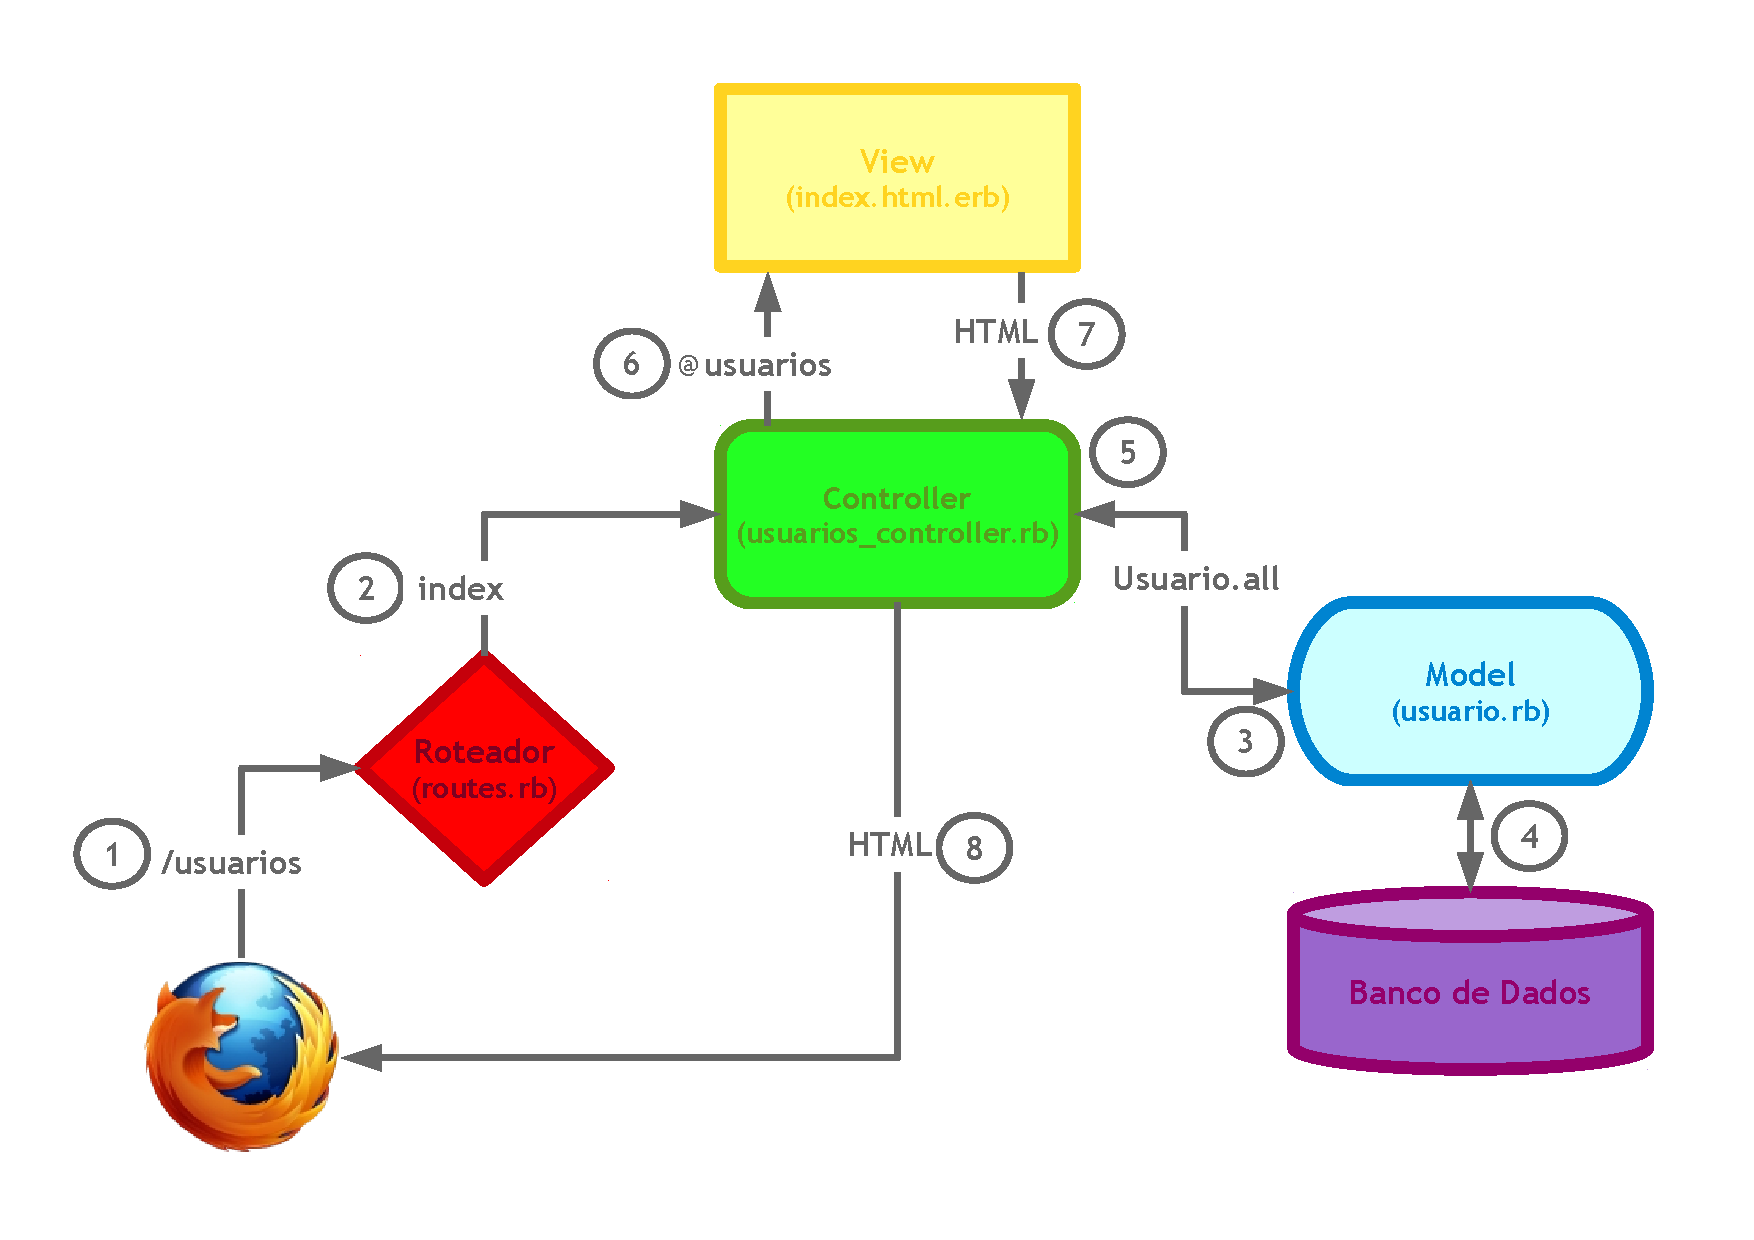
\includegraphics[width=0.70\textwidth]{imagens/mvc-1.pdf}
	\end{figure}
\end{frame}